\documentclass{article}
\usepackage[spanish]{babel}
\usepackage{fancyhdr}
\usepackage{graphicx}
\usepackage{setspace}
\usepackage[table]{xcolor}
\usepackage{tabularx}
\usepackage{array}
\usepackage{multirow}
\usepackage[margin=2.5cm]{geometry}
\usepackage{hyperref}

\pagestyle{fancy}
\lhead{\begin{picture}(0,0) \put(0,-8){
\includegraphics[width=20mm]{img/logoFips.png}} \end{picture}}
\rhead{\begin{picture}(0,0) \put(-25,10){
\includegraphics[width=8mm]{./img/logoAbet.png}} \end{picture}}
\renewcommand{\headrulewidth}{0.5pt}


\fancyhead[C]{
 	\tiny Universidad Nacional de San Agustin de Arequipa \\
  	Facultad de Ingenieria de Produccion y Servicios \\
  	Departamento de Ingenieria de Sistemas e Informatica \\
  	Escuela Profesional de Ingenieria de Sistemas \\
  	\textbf{Programacion Web}
}

\begin{document}
\setstretch{0.75}


\begin{center}
	\Huge \textbf{\\  \Large Laboratorio 01 \\ \Large Tema: Docker}
\end{center}


\begin{figure}[htbp]
  \centering
  
\includegraphics[width=0.4\textwidth]{img/logoUnsa.png}
\end{figure}


\noindent
\renewcommand{\arraystretch}{2}
\begin{table}[h]
\centering
\begin{tabular}{|c|c|c|c|c|c||}
\hline
\multicolumn{1}{|c|}{\textbf{\scriptsize CURSO:}} & \multicolumn{5}{|c|}{\small Programación Web 2} \\ \hline
\multicolumn{1}{|c|}{\textbf{\scriptsize TÍTULO DE LA PRÁCTICA:}} & \multicolumn{5}{|c|}{\small Docker} \\ \hline
\multicolumn{1}{|c|}{\textbf{\scriptsize NRO DE PRÁCTICA:}} & \multicolumn{1}{|c|}{\small 1}& \multicolumn{1}{|c|}{\textbf{\footnotesize AÑO:}} & \multicolumn{1}{|c|}{\small 2024-A} & \multicolumn{1}{|c|}{\textbf{\footnotesize SEMESTRE:}} & \multicolumn{1}{|c|}{\small III Semestre} \\ \hline \multicolumn{1}{|c|}{\textbf{\scriptsize ESTUDIANTE:}} & \multicolumn{5}{|c|}{\small Nina Calizaya Rafael Diego} \\ \hline  \multicolumn{1}{|c|}{\textbf{\scriptsize DOCENTE:}} & \multicolumn{5}{|c|}{\small Ing. Lino Pinto} \\ \hline
\end{tabular}
\end{table}

\clearpage
\begin{center}
	\Huge \textbf{\\ \Large Resolución de la Práctica \\}
\end{center}


\section{Actividades Realizadas}

\subsection{Instalacion de Docker y resolucion de ejercicios pedidos en la practica\\}



apt-get update\\
apt-get install apache2\\
/etc/init.d/apache2 start\\
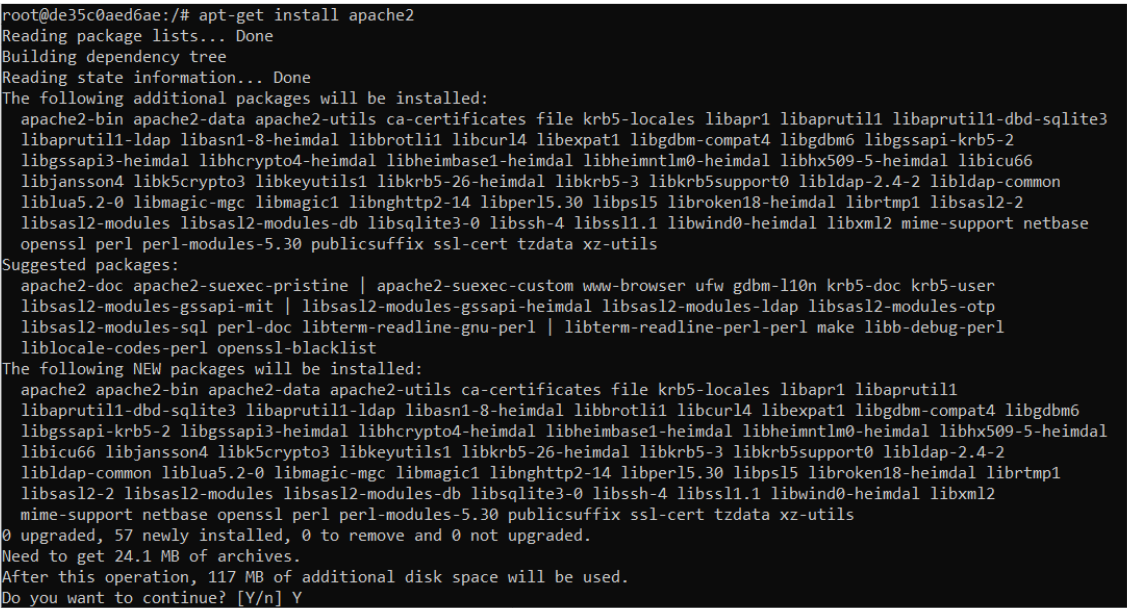
\includegraphics[width=\textwidth]{img/c1.png}
\\
\\
apt-get install vim\\
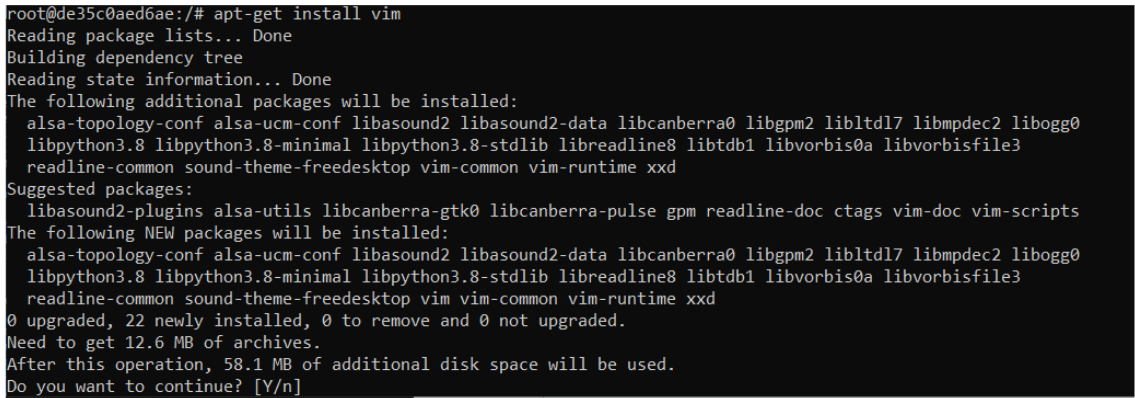
\includegraphics[width=\textwidth]{img/c2.png}
\\
\\
apt-get install libapache2-mod-php7.4\\
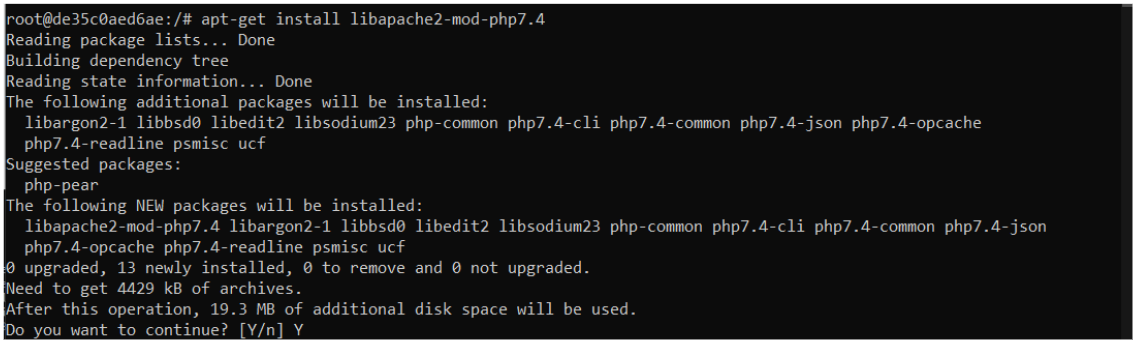
\includegraphics[width=\textwidth]{img/c3.png}
\\
\\
apt-cache search php7.4\\
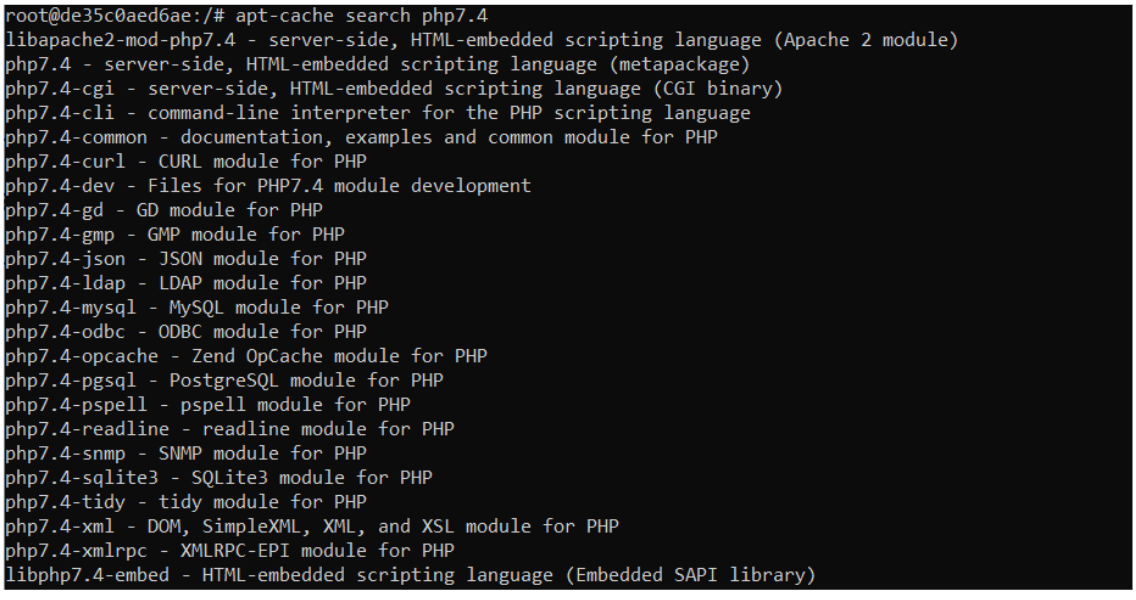
\includegraphics[width=\textwidth]{img/c4.png}
\\
\\
apt-get install openssh-server\\
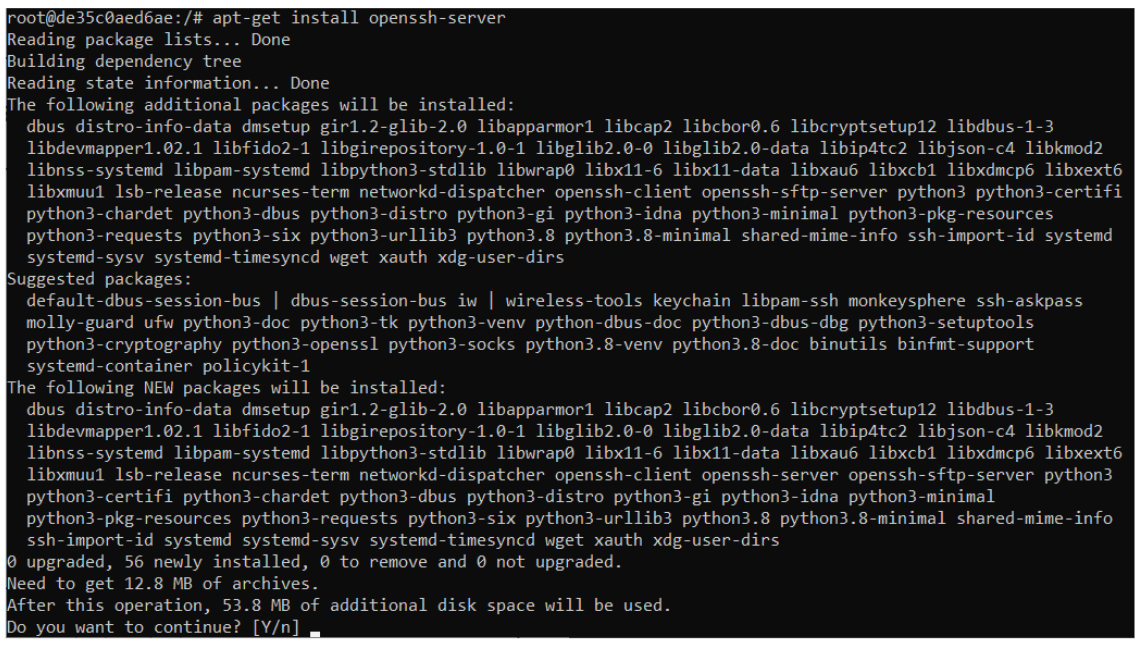
\includegraphics[width=\textwidth]{img/c5.png}
\\
\\
adduser pw2\\
chown -R pw2:www-data /var/www/html/\\
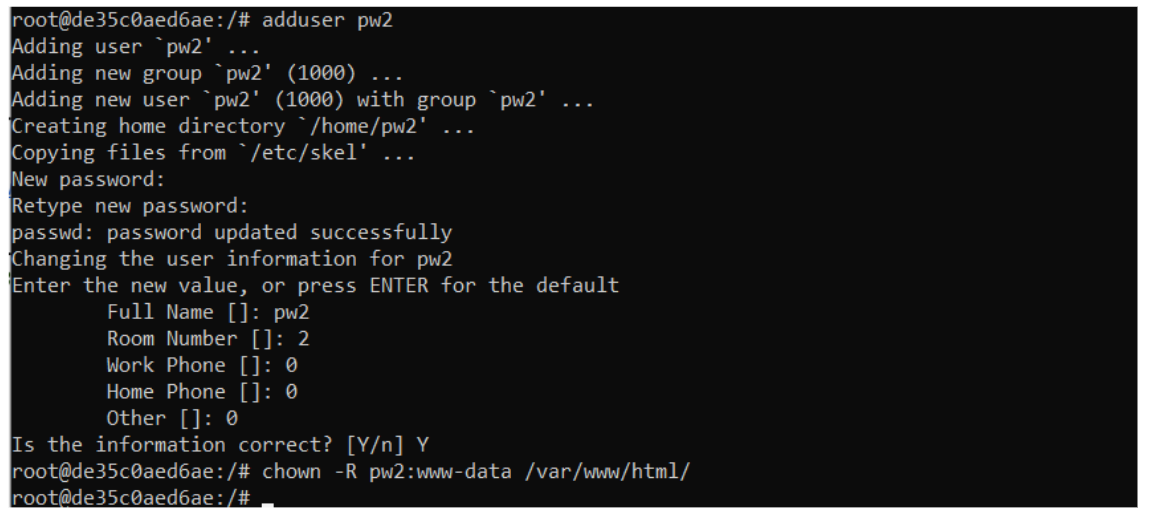
\includegraphics[width=\textwidth]{img/c6.png}
\\
\\
apt-get install mariadb-server\\
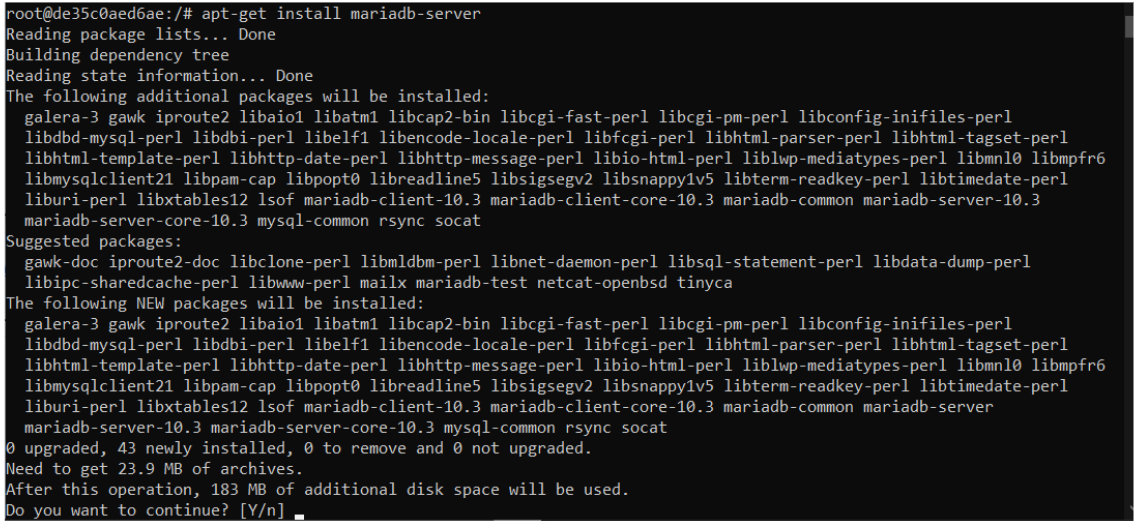
\includegraphics[width=\textwidth]{img/c7.png}
\\
\\
mysql> CREATE USER pw2@localhost IDENTIFIED BY ‘12345678’;\\
myslq> GRANT ALL PRIVILEGES ON menagerie.* TO pw2@localhost;\\
mysql> FLUSH PRIVILEGES;\\
mysql -u pw2 -p\\
password:12345678\\
mysql> SHOW DATABASES;\\
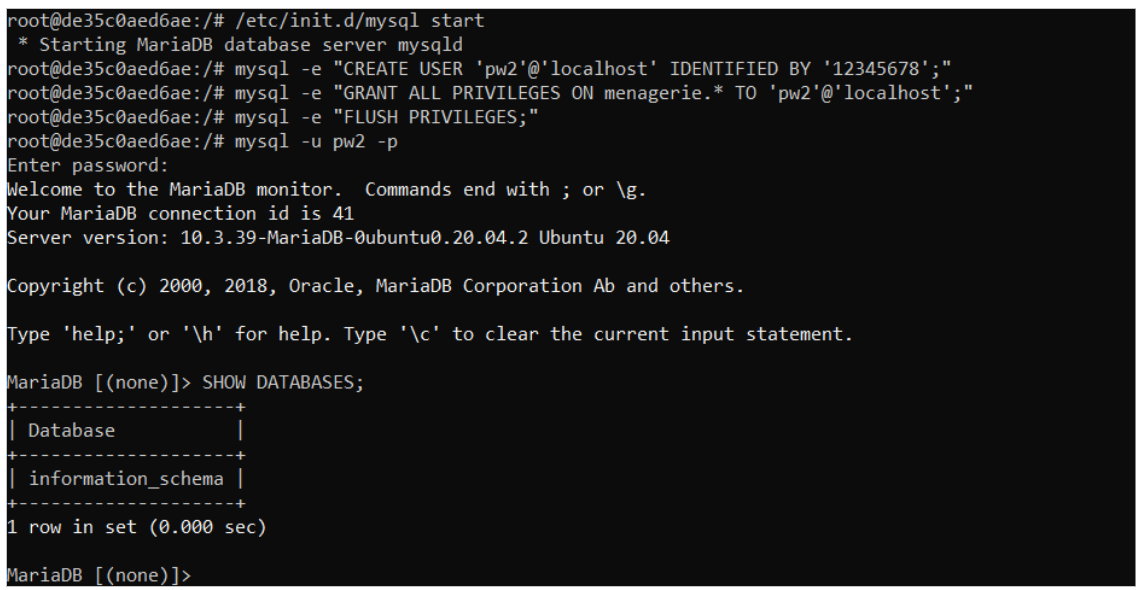
\includegraphics[width=\textwidth]{img/c8.png}
\\
\\
apt-get install perl\\
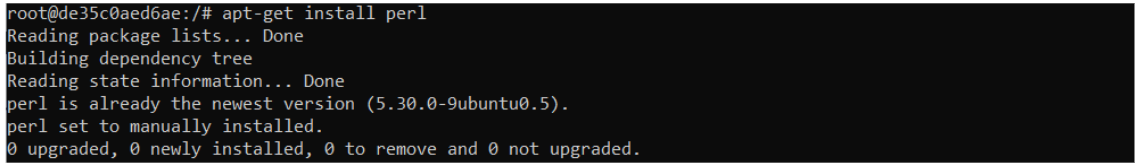
\includegraphics[width=\textwidth]{img/c9.png}
\\
\\
apt-get install libapache2-mod-fcgid\\
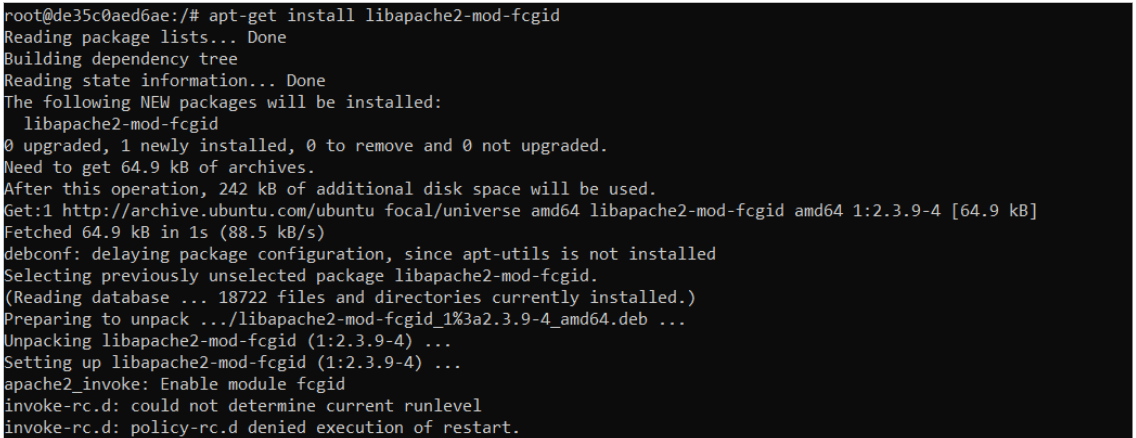
\includegraphics[width=\textwidth]{img/c10.png}
\\
\\
docker cp ./wiki pw2lab01:/var/www/html/\\
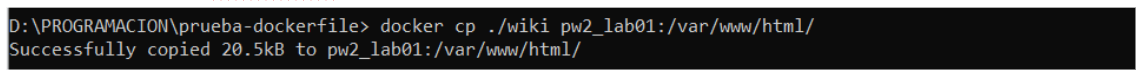
\includegraphics[width=\textwidth]{img/c11.png}


\subsection{Subiendo el proyecto a Docker Hub}

docker build t drn25/pw2textunderscorelab01:latest\\
docker push drn25/pw2textunderscorelab01:latest\\
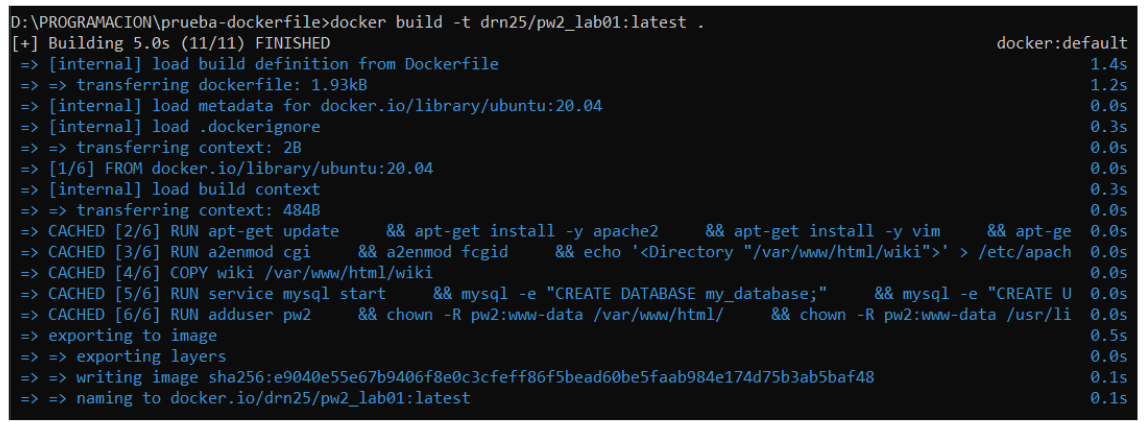
\includegraphics[width=\textwidth]{img/c12.png}\\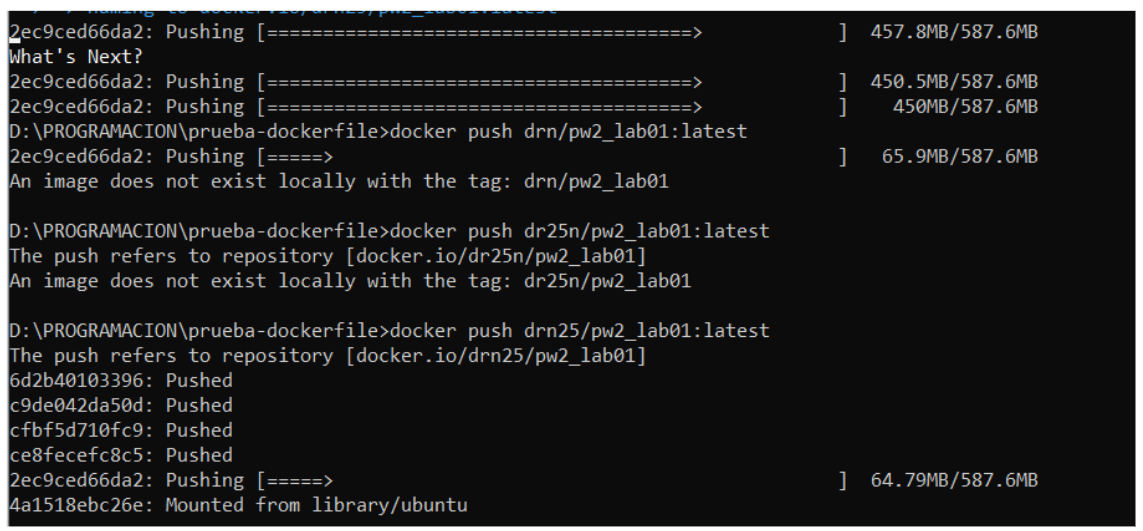
\includegraphics[width=\textwidth]{img/c13.png}
\\
\\

\subsection{Link del video de Docker:}
\url{https://youtu.be/Y0G8sYRPASM}

\subsection{Link del repositorio a Docker Hub}
https://hub.docker.com/layers/drn25/pw2\verb|_|lab01/latest/images/sha256-575aeaece \\ 9a2c6f3077c77f3783b1acacc45da6954030966c66a9c9abbad4a7c?context=repo

\subsection{Link del repositorio a Git Hub}
\url{https://github.com/DrN25/pw2_24a.git}

\end{document}

